
\chapter{Identification}
\label{cha:ident}
In this chapter, the identification process of the controlled system will be
explained. This identification process can be divided in two parts: the data acquisition, where the inputs\slash outputs of the system are
  acquired, and the model identification, where the acquired data is
  used in the identification algorithm, \Autoref{alg:identification}, and the
  identified model is generated.
  
In the next sections this two parts will be described

\section{Data Acquisition}
For the data acquisition, there are some ways to acquire the values of the
inputs\slash outputs, but most of them are divided in two categories, one where
the data is continuously registered, and the other one where the data is buffered
and registered in batches from time to time.
The first one is usually used for online processes, where the continuous flow of
information is necessary, and process that are repeated
extensively, examples of these processes are control loops and failure
detection modules. On the other hand, the second one usually serves for offline
processes, processes that are computationally expensive or happen only once in a
while. Modelling a big system and some more complex control loops can be examples of
such processes. 

Since the
\Autoref{alg:identification} takes as its input a set of paths, all the data is
acquired beforehand, a continuously acquisition is not necessary. The data can
be acquired in batches, and once all the data is collected the algorithm can be
run.

In order to acquire the data from a \PLC{}, the most straightforward way to do
it is by using datalogs. The Siemens \PLC{} S7-1500 includes function blocks to
use inside a \LD{} to store custom data in a \CSV{} formatted file. This file is
saved in a SD card, To retrieve this file, the SD card can be connected to a PC,
or it can be downloaded using a web browser if a Web Server is configured in the
\PLC.




. Section 3.2 of \cite{datalogSiemens}

\subsection{HMI}
\cite{webserverSiemens,userdefinedwebpagesSiemens}
\begin{figure}[H]
  \centering
 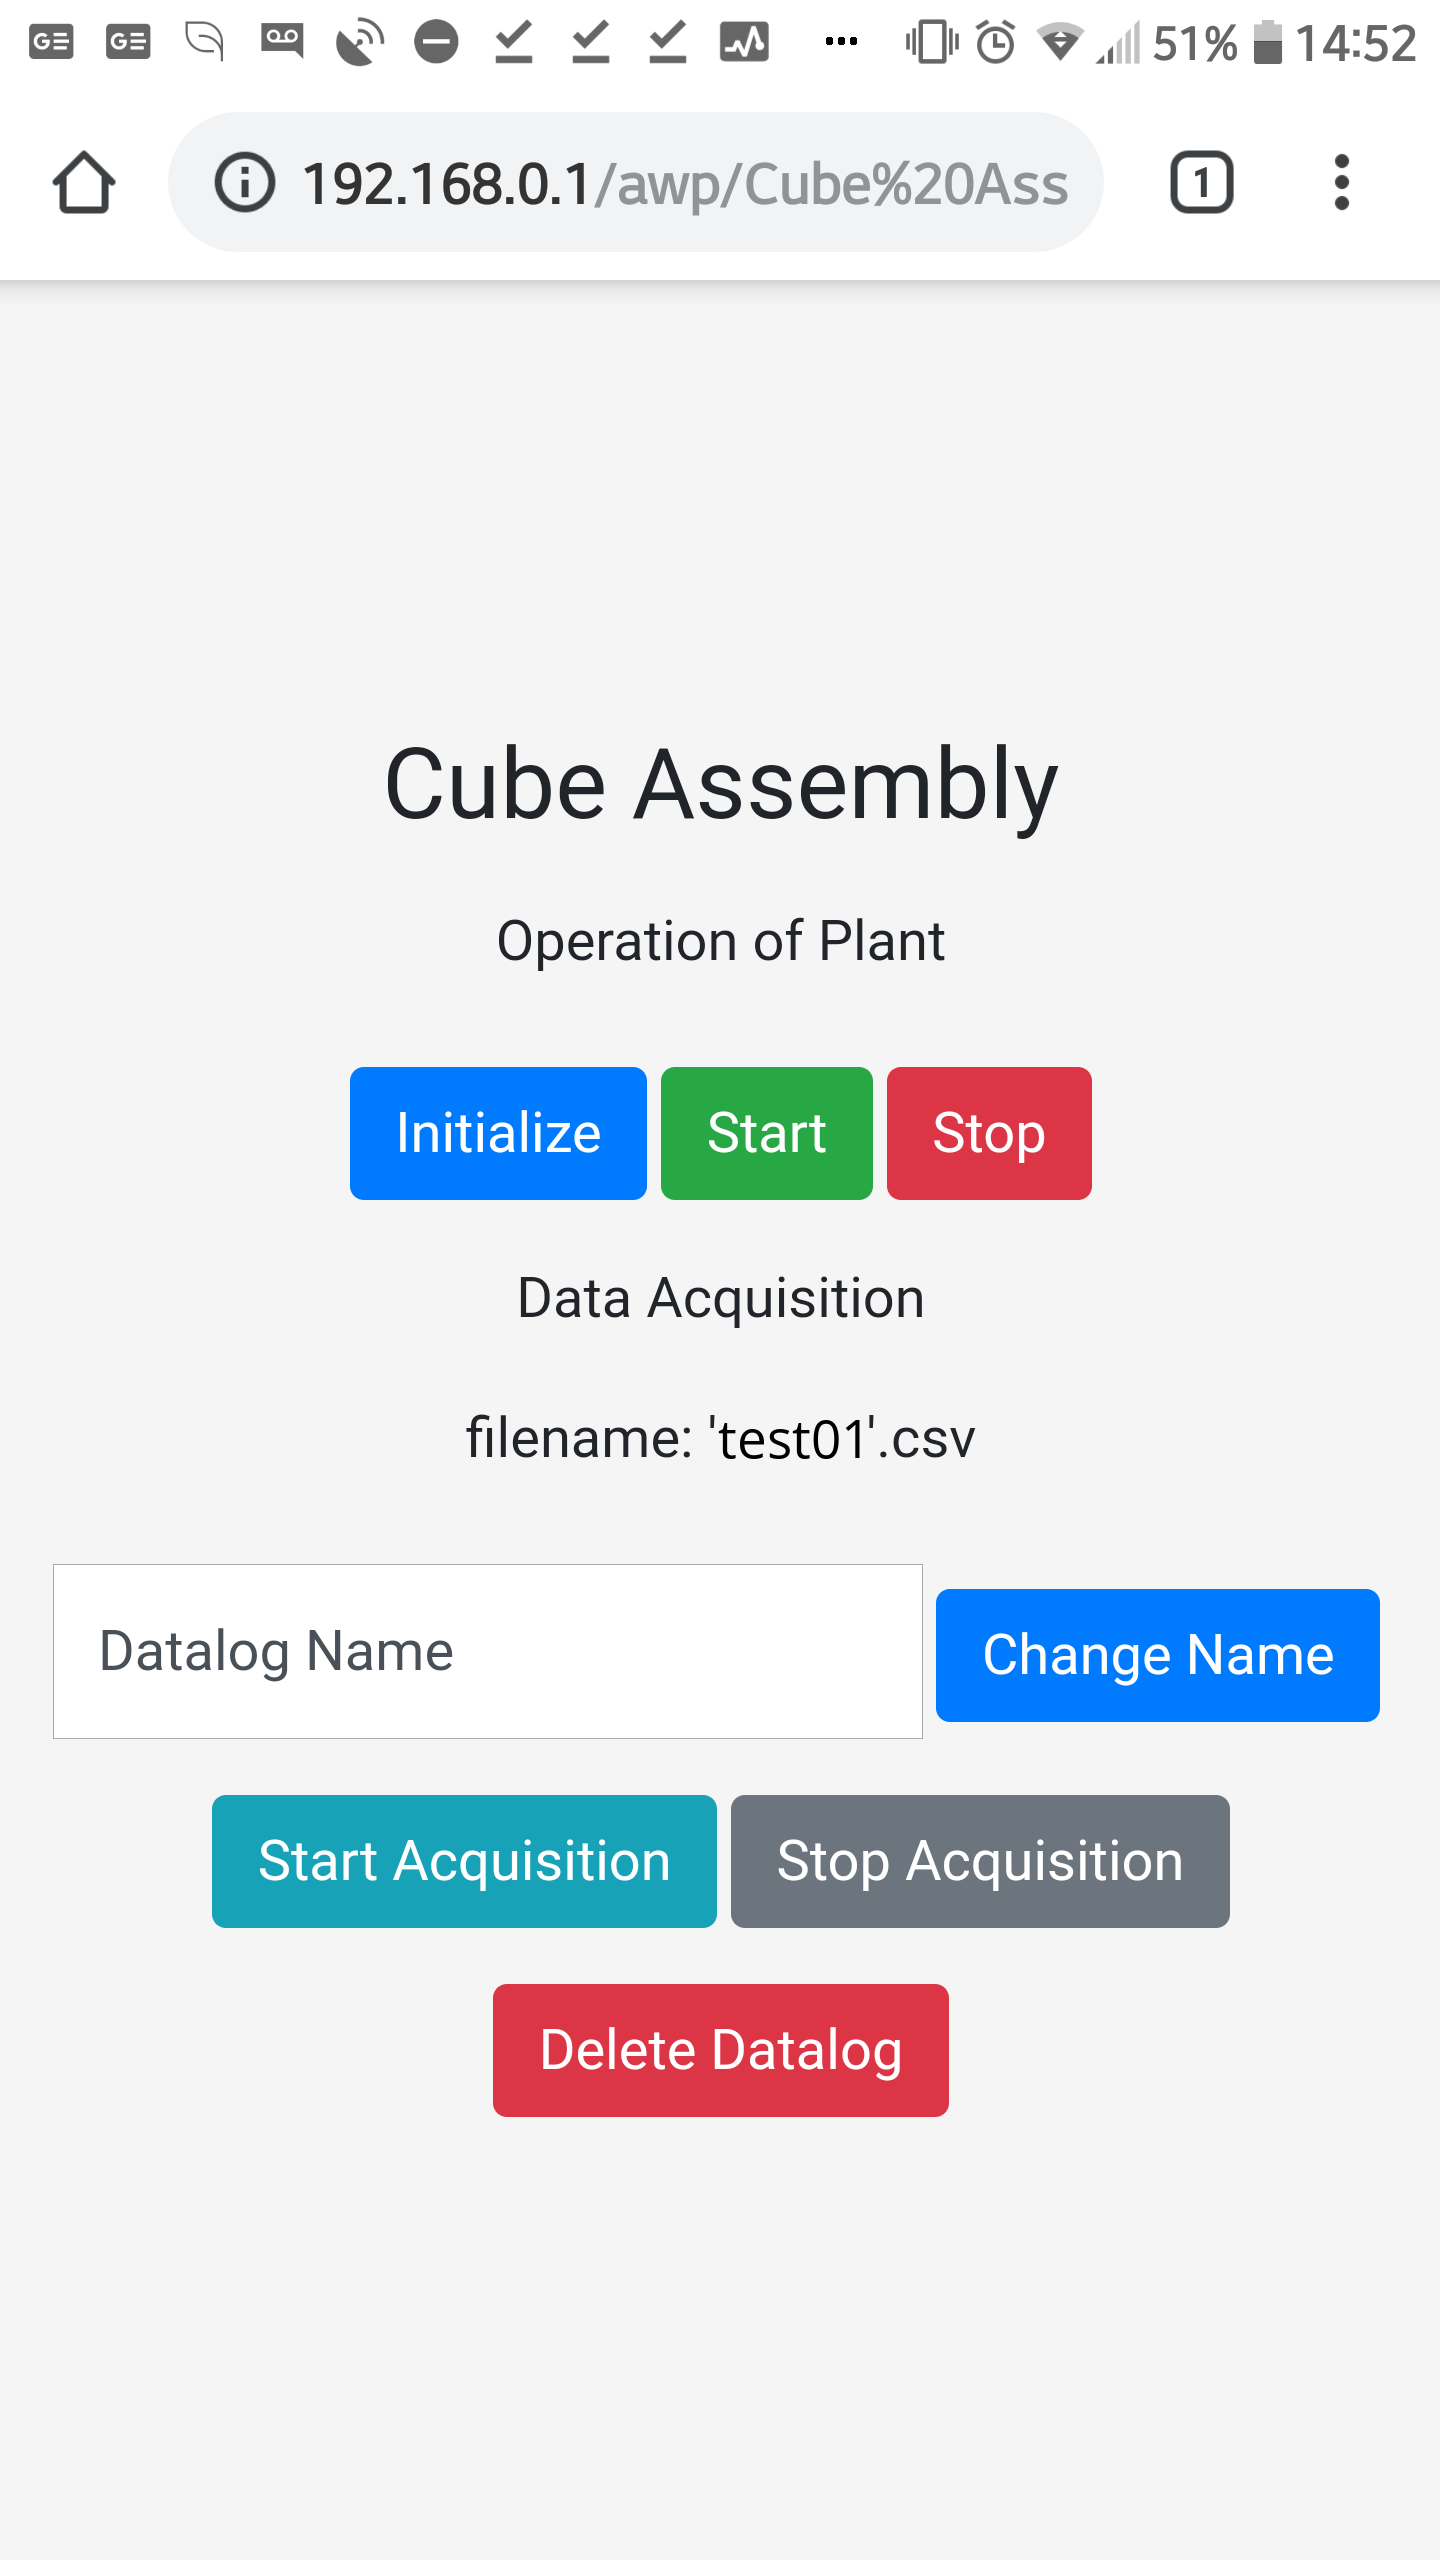
\includegraphics[height=0.6\textwidth]{hmi_mobile2}
  \caption{HMI on mobile.}
  \label{fig:hmi_mobile}
\end{figure}
\section{Model Identification}





%%% Local Variables:
%%% mode: latex
%%% TeX-master: "../monografia"
%%% End: